%\chapterauthor{Author Name}{Author Affiliation}
%\chapterauthor{Second Author}{Second Author Affiliation}
\chapter{Text File Editing}

There are many applications that supports text files or programs editing in Linux, to name a few, \textit{Vim}, \textit{Atom}, \textit{Visual Studio Code}, and many more. These text editors come with different features, and some of them may support advanced functions such as compiling and executing codes.

Among the popular text editors in the Linux community, \textit{Vim} is probably the most popular one that can work in the shell without desktop graphic environment, thus the default built-in text editor for many Linux distributions. \textit{Vim} is introduced in this chapter, followed by some other commonly used text editors.

\section{General Introduction to Vim}

\textit{Vim} is a free and open-source software initially developed by Bram Moolennar, and has become the default text editor of many Unix/Linux based operating systems.

Some people claim \textit{Vim} to be the most powerful text file editor as well as integrated development environment for programming on a Linux machine (and potentially on all computers and servers). The main reasons are as follows.
\begin{itemize}
  \item \textit{Vim} is usually built-in to Linux during the operating system installation, making it the most available and cost-effective text editor.
  \item \textit{Vim} can work on machines where graphical desktop is not supported.
  \item \textit{Vim} is light in size and is suitable to run even on an embedded system.
  \item \textit{Vim} operations are done mostly via mode switch and shortcut keys, so that \textbf{the brain does not need to halt and wait for the hand to grab and move the mouse} which slows down the text editing and interrupts the logic flow.
  \item \textit{Vim} is highly flexible and can be customized according to the user's habit (for example, through \verb|~/.vim/vimrc|), and it allows the users to define shortcut keys.
  \item \textit{Vim} can automate repetitive operations by defining macros.
  \item \textit{Vim} can be integrated with third-party tools for useful functions such as browsing project folders.
\end{itemize}
\textit{Vim} can be come very powerful and convenient for the user if he is very used to it. On the other hand, however, \textit{Vim} is not as intuitive as other text editors such as \textit{gedit} and \textit{notepad++}, and there might be a learning curve for beginners.

\section{Vim Modes} \label{ch:tfe:subsec:vimgeneralintro}

Unlike other text editors, \textit{Vim} defines different ``modes'' during the operation, each mode has some unique features. For example, in the \textit{insert} mode, \textit{Vim} puts keyboard inputs into the text file like an conventional text editor. In the \textit{normal} mode (this is the default mode when opening \textit{Vim}), \textit{Vim} uses useful and customizable shortcut keys to quickly navigate the document and perform operations such as cut, copy, paste, replace, search, and macro functions. In the \textit{virtual} mode, \textit{Vim} allows the user to select partial of the document for further editing. In the \textit{cmdline} mode, \textit{Vim} takes order from command lines and interact with Linux to perform tasks such as save, quit or even navigating folders.

The following Table \ref{ch3tab:vimmodes} summarizes the commonly used modes in Vim.
\begin{table}
  \centering \caption{Commonly used modes in \textit{Vim}.}\label{ch3tab:vimmodes}
  \begin{tabularx}{\textwidth}{lX}
    \hline
    Mode & Description \\ \hline
    Normal & Default mode. It is used to navigate the cursor in the text, search and replace text pieces, and run basic text operations such as undo, redo, cut (delete), copy and paste. \\ \hdashline
    Insert & It is used to insert keyboard inputs into the text, just like commonly used text editors today. \\ \hdashline
    Visual & It is similar to normal mode but areas of text can be highlighted. Normal mode commands can be used on the highlighted text. \\ \hdashline
    Cmdline & It takes in a single line command input and perform actions accordingly, such as save and quit. \\
    \hline
  \end{tabularx}
\end{table}

As a start, the following basic commands can be used to quickly create, edit and save a text file using vim. In home directory, start a shell and key in
\begin{lstlisting}
$ vim testvim
\end{lstlisting}
to create a file named ``testvim'' and open the file using \textit{Vim}. Notice that in some Linux versions, \textit{vi} might be aliased to \textit{vim} by default.

In the opened file, use \verb|Esc| and \verb|i|/\verb|a| to switch between normal mode and insert mode. In the normal mode, use \verb|h|, \verb|j|, \verb|k|, \verb|l| to navigate the position of the cursor. Finally, in the normal mode, use \verb|:w| to save the file, and \verb|:q| to quit \textit{vim}, or use \verb|:wq| to save and quit \textit{Vim}.

The above basic commands and their relationships are summarized in Fig.~\ref{ch3fig:vimbasicmodeswitching}. A flowchart to create/open, edit, save, and quit a text file using the aforementioned commands are given in Fig.~\ref{ch3fig:vimbasicoperationflowchart}.

\begin{figure}
\centering
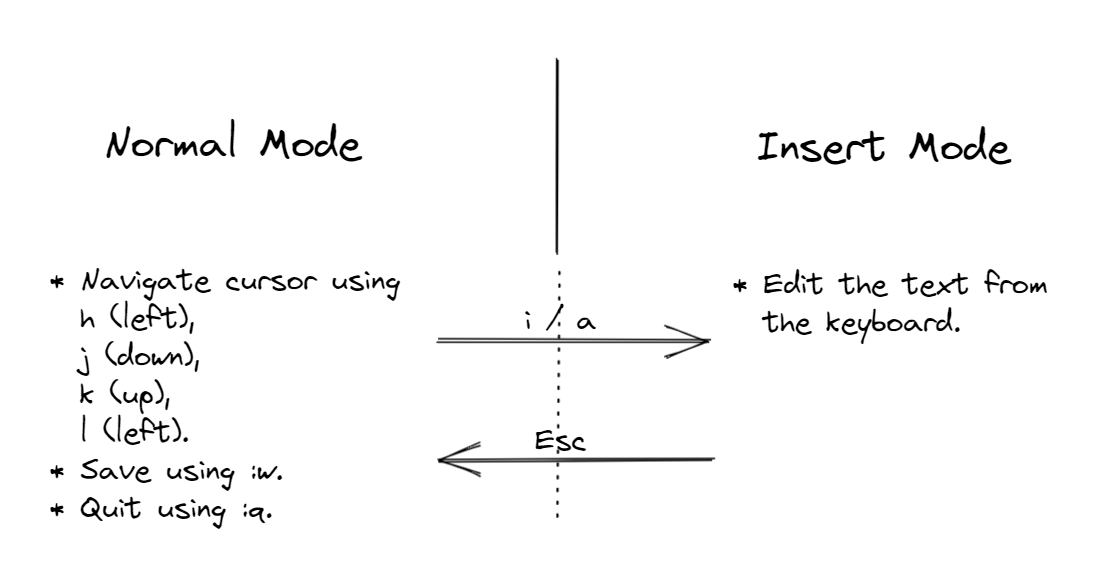
\includegraphics[width=250pt]{chapters/ch_text_file_editing/figures/vimbasicmodeswitching.png}
\caption{Mode switching between normal mode and insert mode, and basic functions associated with the modes.} \label{ch3fig:vimbasicmodeswitching}
\end{figure}

\begin{figure}
\centering
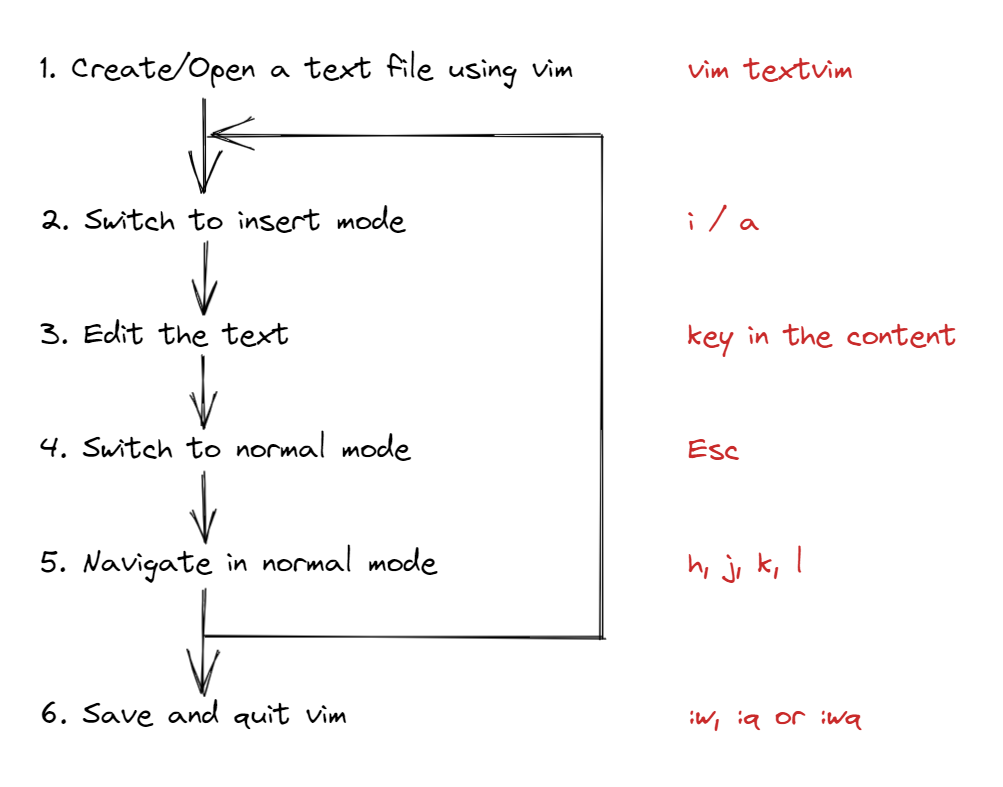
\includegraphics[width=250pt]{chapters/ch_text_file_editing/figures/vimbasicoperationflowchart.png}
\caption{A flowchart for simple creating, editing and saving of a text file using \textit{Vim}.} \label{ch3fig:vimbasicoperationflowchart}
\end{figure}

There are other shortcuts to switch from normal mode to insert mode. Some of them are summarized in Table \ref{ch3tab:switchtoinsert}.

\begin{table}
  \centering \caption{Commonly used shortcuts to switch from normal mode to insert mode.}\label{ch3tab:switchtoinsert}
  \begin{tabularx}{\textwidth}{lX}
    \hline
    Operator & Description \\ \hline
    \verb|i| & Insert before the character at the cursor. \\ \hdashline
    \verb|I| & Insert at the beginning of the row at the cursor. \\ \hdashline
    \verb|a| & Insert after the character at the cursor. \\ \hdashline
    \verb|A| & Insert at the end of the row at the cursor. \\ \hdashline
    \verb|o| & Create a new row below the cursor and switch to insert mode. \\ \hdashline
    \verb|O| & Create a new row above the cursor and switch to insert mode. \\
    \hline
  \end{tabularx}
\end{table}

\section{Vim Profile Configuration}

With the basic operations introduced in Section \ref{ch:tfe:subsec:vimgeneralintro}, we are able to create and edit a text file as we want to, just like using any other text editor. Though at this point the advantages of using \textit{Vim} over other text editors are not obvious yet, the \textit{Vim} editor is at least useable.

Before introducing more advanced features of \textit{Vim} for more convenient user experience, we can now customize the user profile to suit our individual habit. Notice that the customization is completely optional and personal. This section only introduces the ideas and basic methods of such customization, such as re-mapping keys and create user-defined shortcuts. Everything introduced here are merely examples and it is completely up to the user how to design and implement his own profile.

In Linux, navigate to home directory. Create the following path and file \verb|~/.vim/vimrc| or \verb|~/.vimrc|. Open the \textit{vimrc} file as a blank file using \textit{Vim}. The individual user profile can be customized here.

\subsection{Mapping Shortcuts}

It is desirable to re-map some keys to speed up editing. For example, people may want to map \verb|jj| to \verb|Esc| in insert mode for more convenient mode switching to normal mode (consequent ``jj'' is rarely used in English). Other people may feel like mapping \verb|j|, \verb|k|, \verb|i| to \verb|h|, \verb|j|, \verb|k| respectively in normal and visual modes, making the navigation more intuitive. In that case, a different key needs to be mapped for \verb|i| since it is an important key for switching to insert mode.

It is possible re-map certain key (or keys combination) in selected modes. The following configuration in \textit{vimrc} file re-maps the aforementioned keys.
\begin{lstlisting}
inoremap jj <Esc>
noremap j h
noremap J H
noremap k j
noremap K J
noremap i k
noremap I K
noremap h i
noremap H I
\end{lstlisting}
where \verb|inoremap| is used to map keys (combinations) in insert mode, and \verb|noremap| in normal and visual modes.

The upper case letter \verb|S| and lower case letter |s| in control mode are originally used to delete and substitute texts. They may be not so important in practice as there functions are overlapped by another shortcut key \verb|c|, which is powerful in replacing characters and is more frequently used. We can re-map \verb|S| for saving the text, and disable \verb|s| to prevent mis-touching. Similarly, upper case letter \verb|Q| is mapped to quit \textit{Vim}.
\begin{lstlisting}
noremap s <nop>
map S :w<CR>
map Q :q<CR>
\end{lstlisting}
where \verb|<nop>| stands for ``no operation'' and \verb|CR| stands for the ``enter'' key on the keyboard. The keyword \verb|map| differs from \verb|noremap| in the sense that \verb|map| is for recursive mapping.

\subsection{Syntax and Color Scheme}

By default \textit{Vim} displays white color contents on black background. Use the following command in \textit{vimrc} to enable syntax highlighting or change color scheme. Use \verb|:colorscheme| in normal mode in \textit{Vim} to check for available color schemes.
\begin{lstlisting}
syntax on
colorscheme default
\end{lstlisting}

The following command displays the row index and cursor line (a underline at cursor position) of the text, which can become handy during the programming. Furthermore, it sets auto-wrap of text when a single row is longer than the displaying screen.
\begin{lstlisting}
set number
set cursorline
set wrap
\end{lstlisting}

The following command opens a ``menu'' when using cmdline mode, making it easier to key in commands.
\begin{lstlisting}
set wildmenu
\end{lstlisting}

Many users in the community have posted their recommended \textit{Vim} user profile configuration online, such as on \textit{GitHub}. For the convenience of the reader, in the rest of the notebook, we will assume that \textbf{no re-map of keys combinations or shortcuts} are implemented, when introducing the commands.

Notice that the configurations introduced in this section can also be activated with the \textit{Vim} already started. Simply type \verb|:| to switch from normal mode to cmdline mode, then key in the configuration. For example, \verb|:syntax on| to activate the syntax display.

\subsection{Plug Tools}

In the Linux community, many plug tools have created to add useful features for \textit{Vim}. As a demonstration, in this section \textit{vim-plug}, a light-size vim plugin management tool created on GitHub, is used to install selected \textit{Vim} plugins. Details about \textit{vim-plug} can be found at GitHub under \textit{junegunn/vim-plug}.

Following the instruction given by GitHub under \textit{junegunn/vim-plug}, to use \textit{vim-plug} on Linux, the very first step is to use \textit{cURL}, a command-line tool for transferring data specified with URL syntax (very likely to be built-in to the user's Linux distribution), to download \textit{vim-plug}. To confirm \textit{cURL} installation, use the following command in Linux shell
\begin{lstlisting}
$ apt-cache policy curl
\end{lstlisting}
and if \textit{cURL} is installed, the shell is expected to return somthing like
\begin{lstlisting}
curl:
  Installed: 7.68.0-1ubuntu2.7
  Candidate: 7.68.0-1ubuntu2.7
  Version table:
 *** 7.68.0-1ubuntu2.7 500
        500 http://cn.archive.ubuntu.com/ubuntu focal-updates/main amd64 Packages
        500 http://security.ubuntu.com/ubuntu focal-security/main amd64 Packages
        100 /var/lib/dpkg/status
     7.68.0-1ubuntu2 500
        500 http://cn.archive.ubuntu.com/ubuntu focal/main amd64 Packages
\end{lstlisting}

With \textit{cURL} installed, use the following in the shell to install \textit{vim-plug}
\begin{lstlisting}
$ curl -fLo ~/.vim/autoload/plug.vim --create-dirs \
    https://raw.githubusercontent.com/junegunn/vim-plug/master/plug.vim
\end{lstlisting}

In the beginning \textit{vimrc}, add the following to indicate the plugins to be installed. Here as an example, \textit{vim-airline/vim-airline} and \textit{joshdick/onedark.vim} are installed, the first of which adds a status line at the bottom of the \textit{Vim} window, and the second adds a popular color scheme ``onedark''.
\begin{lstlisting}
call plug#begin()
Plug 'vim-airline/vim-airline'
Plug 'joshdick/onedark.vim'
call plug#end()
\end{lstlisting}

Finally, reload \textit{vimrc}, then run \verb|:PlugInstall| in cmdline mode to install the plugins.

\section{Basic Operations in Vim}

In normal mode, the most frequently used operation is probably \verb|u|, which stands for undo. Other commonly used operations, such as delete, cut, copy, paste, replace and search, are mostly done in normal mode through shortcut keys. For example, \verb|dd| delete (cut) the entire row at the cursor and \verb|p| paste the content in the clipboard to the cursor position. For beginners, remembering shortcut keys can be difficult. In such case, it is suggested looking for the consistent patterns of the different commands, instead of brute-force remembering the operations.

Many \textit{Vim} shortcut keys in normal mode has the following structure, namely an operator command followed by a motion command, as shown below.
\begin{lstlisting}
<operator><motion>
\end{lstlisting}
The operator command tells \textit{Vim} what to do (say, copy), and the motion command tells the applicable range of the operation (say, a row, or a word, or a character). Some operator commands may work alone without motion commands.

\subsection{Cut, Change, Copy and Paste}

The following lines taken from Wikipedia under ``William Shakespeare'' is used as an example to demonstrate delete/cut, change, copy and paste functions. In the text file, each sentence takes a new row as given by Figure \ref{ch3fig:vimdemo1}.

\begin{shortbox}
William Shakespeare (bapt. 26 April 1564 – 23 April 1616) was an English playwright, poet and actor, widely regarded as the greatest writer in the English language and the world's greatest dramatist.

He is often called England's national poet and the ``Bard of Avon'' (or simply ``the Bard'').
\end{shortbox}

\begin{figure}
\centering
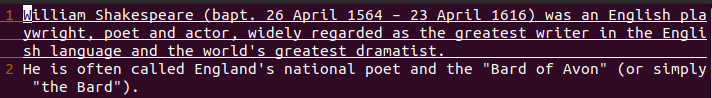
\includegraphics[width=250pt]{chapters/ch_text_file_editing/figures/vimdemo1.png}
\caption{A piece of text of ``William Shakespeare'', for demonstration.} \label{ch3fig:vimdemo1}
\end{figure}

To quickly delete/cut a single character, use either \verb|x| and \verb|X| to delete the character at the cursor and previous to the cursor respectively. In summary, \verb|x| and \verb|X| play like \verb|delete| and \verb|backspace| respectively in other text editors.

To delete multiple characters, one way is to press \verb|x| or \verb|X| multiple times. Alternatively, it is possible for \textit{Vim} to automatically repeat the procedure. For example, \verb|20x| tells \textit{Vim} to perform \verb|x| for 20 times. The same applies for other operators or motions commands. For example, \verb|10l| executes \verb|l| for 10 times, making the navigation faster.

Operator \verb|d| also deletes the contents of the text, but it requires a motion command and can be used more flexibly. The motion shall tell \textit{Vim} what to delete/cut.

For example, \verb|dl| deletes one character to the right, i.e. deletes the character at the cursor just like \verb|x|. Likewise, \verb|dh| deletes one character to the left just like \verb|X|. Similarly, \verb|d20l| deletes 20 characters to the right, where ``20l'' as a whole plays as the motion of ``20 characters to the right''. A combination by using things like \verb|5d4l| also works, since $20=5\times 4$.

Command \verb|d| can be used even more flexibly. For example, by using word-related motions, \verb|d| can delete/cut by words instead of by characters. Move the cursor to the beginning of a word, (for example, ``S'' in ``Shakespeare''), use \verb|dw| to delete the word. The word motion \verb|w| is similar with \verb|l|, except that \verb|l| directs to the next character, while \verb|w| directs to the beginning of next word. Similarly, \verb|b| directs to the beginning of the current/previous word. Thus, \verb|db| can be used to delete word to the left. Examples \verb|d10b|, \verb|10db|, \verb|d20w|, \verb|5d4w| can be used to delete multiple words at a time. Motions \verb|w| and \verb|b| can also be used to navigate in the text just like \verb|l| and \verb|h|.

When in the middle of a word, \verb|dw| will delete the characters from the cursor to the beginning character of the next word. For example, if the cursor is currently at ``k'' in ``Shakespeare'', \verb|dw| will delete ``kespeare '' (notice that the space between ``Shakespeare'' and ``(bapt.'' will also be deleted). To delete from the beginning of the word instead, you can use \verb|b| first to navigate back to the beginning of the word. Alternatively, use ``inner-word'' motion \verb|iw| to indicate that the whole word of the cursor shall be deleted.

In addition to character-related motions \verb|h|, \verb|l| and word-related motions  \verb|b|, \verb|w|, there are similar motions for sentence \verb|(| (previous), \verb|)| (next) and paragraph \verb|{| (previous), \verb|}| (next). There are also inner-sentence motion \verb|is|, inner-paragraph motion \verb|ip|, inner-quotation motion \verb|i'|, \verb|i"|, \verb|i`| and inner-block motion \verb|i(|, \verb|i<|, \verb|i{|, and many more. For example, when the cursor is at ``A'' of ``26 April 1564'', \verb|di(| will delete everything inside ``()'', i.e. deleting ``bapt. 26 April 1564 - 23 April 1616''.

To conclude, the operators and motions introduced so far are listed in Tables \ref{ch3tab:deletecut} and \ref{ch3tab:motion}. Notice that motions \verb|aw|, \verb|as|, \verb|ap| are also given in the table. They are similar with their corresponding \verb|iw|, \verb|is|, \verb|ip| except that when deleting, the consequent blank space (for word and sentence) or blank row (for paragraph) will also be deleted.

\begin{table}
  \centering \caption{Commonly used operators related to delete/cut, change, copy and paste.}\label{ch3tab:deletecut}
  \begin{tabularx}{\textwidth}{lX}
    \hline
    Operator & Description \\ \hline
    \verb|x| & Delete/Cut the character at cursor. \\ \hdashline
    \verb|X| & Delete/Cut the character before cursor. \\ \hdashline
    \verb|dd| & Delete/Cut the entire row. \\ \hdashline
    \verb|d| & Delete/Cut selected text according to the motion command. \\ \hdashline
    \verb|cc| & Change the entire row. \\ \hdashline
    \verb|c| & Change selected text according to the motion command. \\ \hdashline
    \verb|yy| & Copy the entire row. \\ \hdashline
    \verb|y| & Copy selected text according to the motion command. \\ \hdashline
    \verb|p| & Paste clipboard to the cursor. \\
    \hline
  \end{tabularx}
\end{table}

\begin{table}
  \centering \caption{Commonly used motions.}\label{ch3tab:motion}
  \begin{tabularx}{\textwidth}{lX}
    \hline
    Motion & Description \\ \hline
    \verb|h|, \verb|l| & One character to the left or right. \\ \hdashline
    \verb|j|, \verb|k| & One row to the up or down. \\ \hdashline
    \verb|b|, \verb|w| & One word to the previous or next. \\ \hdashline
    \verb|(|, \verb|)| & One sentence to the previous or next. \\ \hdashline
    \lstinline{\{}, \lstinline{\}} & One paragraph to the previous or next. \\ \hdashline
    \verb|iw|, \verb|is|, \verb|ip| & inner-word, inner-sentence, inner-paragraph. \\ \hdashline
    \verb|aw|, \verb|as|, \verb|ap| & a word, a sentence, a paragraph (including the end blank). \\ \hdashline
    \verb|i'|, \verb|i"|, \verb|i`| & inner-quotation for different types of quotations. \\ \hdashline
    \verb|i(|, \verb|i<|, \verb|i[|, \lstinline{\}} & inner-block for different types of brackets. \\ \hdashline
    \verb|0| & Beginning of the row. \\ \hdashline
    \verb|$| & Ending of the row. \\ \hdashline
    \verb|gg| & Beginning of the text. \\ \hdashline
    \verb|G| & Beginning of the last row of the text. \\
    \hline
  \end{tabularx}
\end{table}

To change contents, use operator \verb|c|, which works the same way as \verb|d| but it automatically switch to insert mode at where the content is removed.

To copy a piece of text to clipboard, use \verb|y| (stands for ``yank'') followed by its associated motion to indicate the range of text. The motions also follow Table \ref{ch3tab:motion}.

To paste the text in the clipboard to the cursor, use \verb|p|. No motion is required.

In addition Table \ref{ch3tab:motion}, another commonly used type of motion is to ``find by character''. For example, consider the following row of text. The cursor is currently at letter ``A''.
\begin{lstlisting}
ABCDEFG;HIJKLMN;OPQ;RST;UVW;XYZ
\end{lstlisting}
In normal mode, using \verb|f| followed by a character will navigate the cursor to the nearest corresponding character that appears in the text. For example, \verb|fG| will move the cursor to letter ``G''. Similarly, \verb|f;| will move the cursor to the ``;'' between ``G'' and ``H''. Key in \verb|f;| again and the cursor will move to ``;'' between ``N'' and ``O''. From here key in \verb|2f:| and the cursor will go to ``;'' between ``T'' and ``U'', as it is equivalent to executing \verb|f;| twice. If \verb|df;| is used when the cursor is at letter ``A'', ``ABCDEFG;'' will be deleted.

\subsection{Search in the Text}

It is common to search and highlight a particular word or phrase in the text. To make the searching result highlighted, add the following line to the user profile \textit{vimrc}.
\begin{lstlisting}
set hlsearch
exec "nohlsearch"
set incsearch
set ignorecase
\end{lstlisting}
where \verb|hlsearch| enables highlighting all matching results in the text, and \verb|incsearch| enables highlighting texts as the keyword is keying in. \textit{Vim} remembers the keyword from the previous search and may automatically hight them in the text on a new session, which can be problematic sometimes. The command \verb|exec "nohlsearch"| (\verb|exec| command in the user profile make \textit{Vim} execute that command when starting a new session) that comes after \verb|set hlsearch| resolves this issue by forcing \textit{Vim} to clear its memory. Finally, \verb|ignorecase| allows case insensitive while searching.

In normal mode, use \verb|/<keyword>| to search keywords or phrase. With the above setup, searching for ``he'' using \verb|/he| leads to the following result given in Fig.~\ref{ch3fig:vimdemo2}.
\begin{figure}
\centering
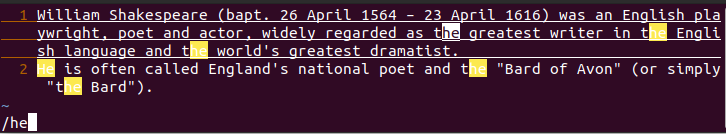
\includegraphics[width=250pt]{chapters/ch_text_file_editing/figures/vimdemo2.png}
\caption{Search ``he'' in the piece of text of ``William Shakespeare''.} \label{ch3fig:vimdemo2}
\end{figure}
From Fig.~\ref{ch3fig:vimdemo2}, it can be seen that all appearances of ``he'' (case insensitive) is highlighted, and the cursor is automatically moved to its first appearance, i.e. ``he'' in ``and the world's greatest dramatist''. Click \verb|Enter| to confirm the searching content. Use \verb|n| and \verb|N| to navigate the cursor from the highlighted results. Notice that at this point, \verb|n| and \verb|N| can be used as motion together with delete/cut, change and copy as given in Table \ref{ch3tab:deletecut}.

To quit searching, use \textit{cmdline} command \verb|:nohlsearch| in normal mode and the highlights shall be gone. For convenience, people may prefer to map it with a customized shortcut key as well, for example in \textit{vimrc} use
\begin{lstlisting}
noremap <Space> :nohlsearch<CR>
\end{lstlisting}
so that \verb|Space| can be used to clear the search highlights.

\section{Visual Modes of Vim}

The use of a mouse makes selecting a block of text very intuitive. In most text editors, the selected text will be highlighted, as if the cursor expands from one character to the entire block of text. Sequentially, operations such as delete and copy can be performed on the selected text.

The three visual modes of \textit{Vim}, namely ``visual'', ``visual-line'' and ``visual-block'', provide similar experience where the user can select and highlight a block of text.

Use \verb|v| to enter the visual mode, then navigate the cursor to select a block of text. This allows the user to select text between any two characters. An example is given by Fig. \ref{ch3fig:vimvm1}. Alternatively, use \verb|V| to enter the visual-line mode where multiple lines can be easily selected, and use \verb|<ctrl>+v| to enter visual-block mode to select a rectangular block of text.

\begin{figure}
	\centering
	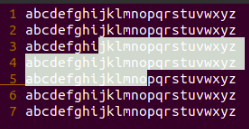
\includegraphics[width=100pt]{chapters/ch_text_file_editing/figures/vimvm1.png}
	\caption{An example of visual mode where a block of text is selected.} \label{ch3fig:vimvm1}
\end{figure}

In any of the above visual mode, use \verb|:normal + <operation>| to execute operation(s) form the normal mode. This allows convenient editing of multiple lines of text all together.

\section{Vim Macros}

\textit{Vim} macros can become handy for frequent and repetitive works.

...

\section{Other Text Editors}

Apart from \textit{Vim}, many other text editors are also widely used in Linux, each with different features. For demonstration purpose, \textit{Vim} and other text editors are used to open a bash shell script that calculates the first 10 elements of fibonacci series.

\begin{figure}
	\centering
	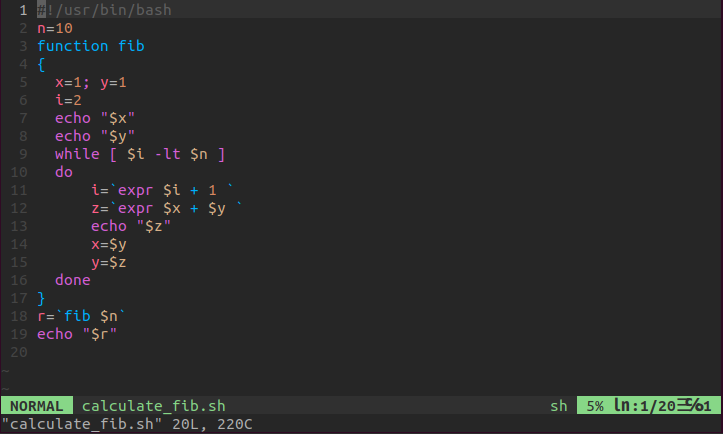
\includegraphics[width=4in]{chapters/ch_text_file_editing/figures/vim_fib.png}
	\caption{\textit{Vim} (with user's profile customization as introduced in this chapter).}
\end{figure}

\begin{figure}
	\centering
	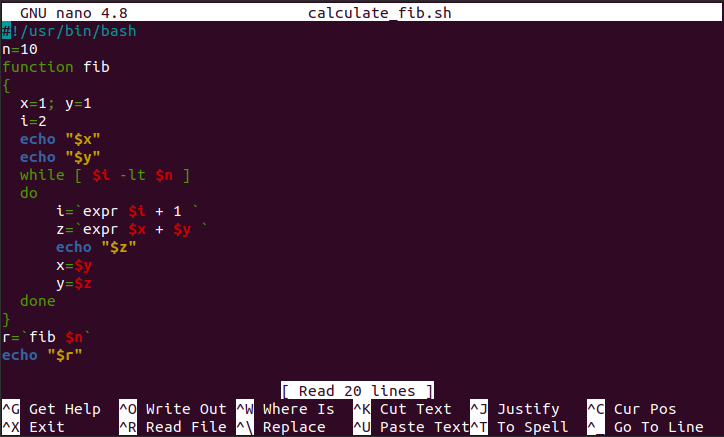
\includegraphics[width=4in]{chapters/ch_text_file_editing/figures/nano_fib.png}
	\caption{\textit{Nano}.}
\end{figure}

\begin{figure}
	\centering
	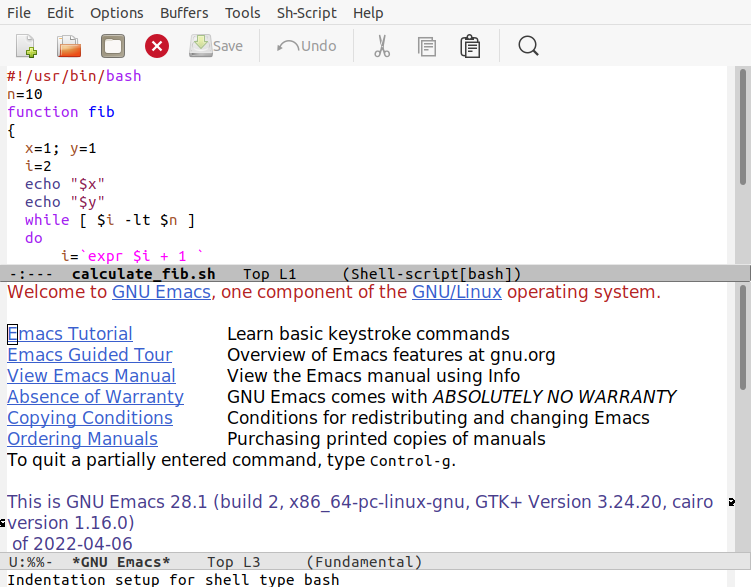
\includegraphics[width=4in]{chapters/ch_text_file_editing/figures/emacs_fib.png}
	\caption{\textit{Emacs}.}
\end{figure}

\begin{figure}
	\centering
	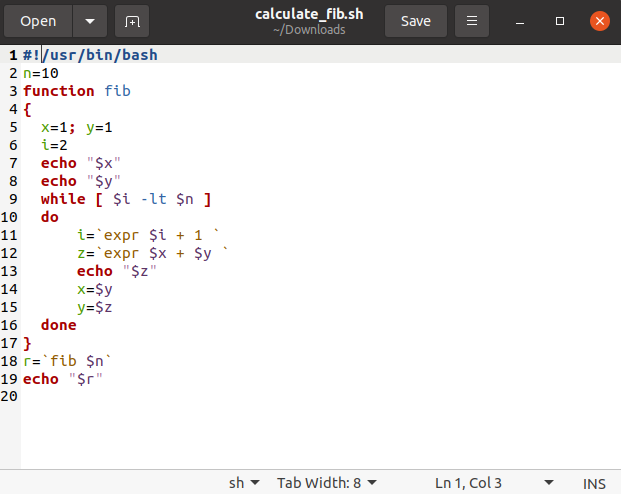
\includegraphics[width=4in]{chapters/ch_text_file_editing/figures/gedit_fib.png}
	\caption{\textit{Gedit}.}
\end{figure}

\begin{figure}
	\centering
	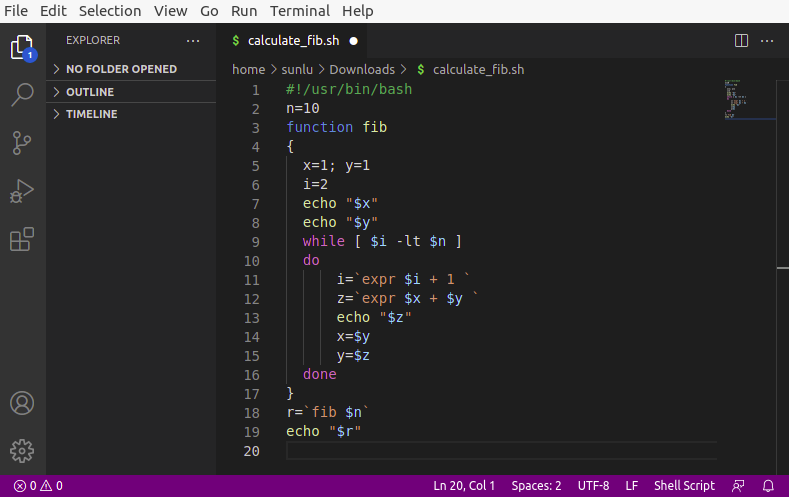
\includegraphics[width=4in]{chapters/ch_text_file_editing/figures/vscode_fib.png}
	\caption{\textit{Visual Studio Code}.}
\end{figure}

\begin{figure}
	\centering
	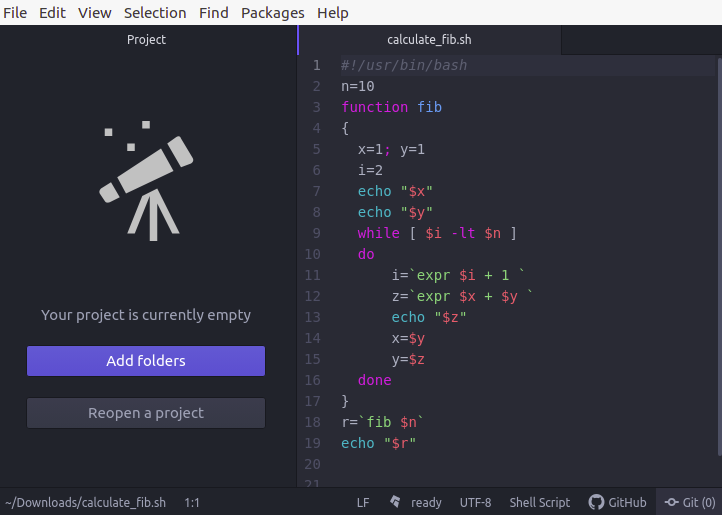
\includegraphics[width=4in]{chapters/ch_text_file_editing/figures/atom_fib.png}
	\caption{\textit{Atom}.}
\end{figure}

















